\section{Introduction} \label{sec:intro}

Unsupervised part-of-speech (POS) induction aims to classify words
into syntactic categories using unlabeled, plain text input.  The
problem of induction is important for studying under-resourced
languages that lack labeled corpora and high quality dictionaries.  It
is also essential in modeling child language acquisition because every
child manages to induce syntactic categories without access to labeled
sentences, labeled prototypes, or dictionary constraints
\cite{ambridge2011child}.  Categories induced from data may point to
shortcomings or inconsistencies of hand-labeled categories as
discussed in Section~\ref{sec:discuss}.  Finally, the induced
categories or the vector representations generated by the induction
algorithms may improve natural language processing systems when used
as additional features.

Word-based POS induction systems classify different instances of a
word in a single category (which we will refer to as the {\em
  one-tag-per-word assumption}).  Instance-based systems classify each
occurence of a word separately and can handle ambiguous words.

Examples of word-based systems include ones that represent each word
with the vector of neighboring words (context vectors) and
cluster them
\cite{Schutze:1995:DPT:976973.976994,lamar-EtAl:2010:Short,Lamar:2010:LCU:1870658.1870736},
use a prototypical bi-tag HMM that assigns each word to a latent
class
\cite{Brown:1992:CNG:176313.176316,Clark:2003:CDM:1067807.1067817},
restrict a HMM based Pitman-Yor process to perform one-tag-per-word
inference \cite{blunsom-cohn:2011:ACL-HLT2011}, define a word-based
Bayesian multinomial mixture model
\cite{christodoulopoulos-goldwater-steedman:2011:EMNLP}, or construct
word vector representations based on co-occurrences with contextual
features \cite{yatbaz-sert-yuret:2012:EMNLP-CoNLL}.

\begin{figure}[t] \centering
  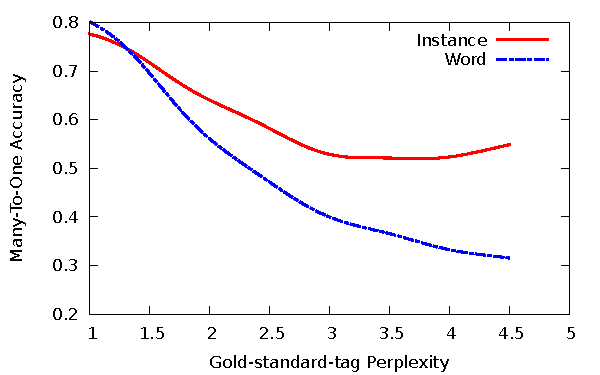
\includegraphics[width=.7\textwidth]{ksmooth-f.pdf} 
  \caption{The accuracy comparison of word and instance based
    part-of-speech induction models as a function of target word
    ambiguity (as measured by gold-standard-tag perplexity described
    in Section~\ref{sec:typevsinstance}) on the Penn Treebank.}
  \label{fig:perplexity}
\end{figure}

The obvious limitation of the one-tag-per-word assumption is that
instances of ambiguous words that have more than one POS role are
grouped into the same class.  For example, the word {\em offer} is
tagged as NN(399), VB(105) and VBP(34)\footnote{NN, VB and VBP are
  three POS tags from the Penn Treebank corpus and they correspond to
  singular noun, verb in base form and non-$3^{rd}$person singular
  verb in present tense, respectively.  The numbers in parentheses are
  the frequencies.} in its 538 occurrences in the human labeled Wall
Street Journal (WSJ) Section of the Penn Treebank (PTB) corpus
\cite{treebank3}.  If all instances of {\em offer} are assigned to the
most frequent tag NN, 36\% (139/538) will be erroneously labeled.  In
spite of this shortcoming, word-based POS induction systems generally
do well because the one-tag-per-word assumption is mostly accurate:
93.69\% of the word occurrences are tagged with their most frequent
POS tag in the PTB \cite{Toutanova:2003:FPT:1073445.1073478}.

In order to handle ambiguous words, models without a strict
one-tag-per-word assumption need to group word {\em instances} into
clusters according to their contexts.  Some of these instance-based
models bias words to have few tags using sparse priors in a Bayesian
setting
\cite{goldwater-griffiths:2007:ACLMain,johnson:2007:EMNLP-CoNLL2007,Gao:2008:CBE:1613715.1613761},
or posterior regularization \cite{Ganchev:2010:PRS:1859890.1859918}.
Sch\"{u}tze \shortcite{SchutzePe93} represents the context of a word
instance by concatenating context vectors of its left and right
neighboring words, and clusters word instances.  Berg-Kirkpatrick et
al.  \shortcite{bergkirkpatrick-klein:2010:ACL} use an EM algorithm
where they replace the multinomial components with miniature logistic
regressions and achieve the highest instance-based accuracy on PTB.
Christodoulopoulos et al.
\shortcite{Christodoulopoulos:2010:TDU:1870658.1870714} select
prototypes of each cluster from the output of Brown
\shortcite{Brown:1992:CNG:176313.176316} and feed them to a HMM model
that can handle prototypes as features
\cite{Haghighi:2006:PLS:1220835.1220876}.  However none of these
models achieve results comparable to the best word-based systems.  

In this work, we show that one can build an instance-based system that
can perform significantly better on highly ambiguous words (see
Figure~\ref{fig:perplexity}) and yet is competitive with word-based
systems in overall accuracy.

We follow the state of the art word-based system
\cite{yatbaz-sert-yuret:2012:EMNLP-CoNLL} and use probable substitutes
of a word instance as its contextual features.  The following examples
illustrate how such paradigmatic (substitute based) contextual
features can capture the similarity between two contexts where a
syntagmatic (neighbor based) representation would fail:

\begin{quotation}
(1) {\em ``Pierre Vinken, 61 years old, will join the board
  as a nonexecutive {\bf director} Nov.~29.''} 
\\ director $\rightarrow$ chairman
(.8242), director (.0127), directors (.0127) $\ldots$

(2) {\em ``$\ldots$ Joseph Corr was succeeded by Frank
  Lorenzo, {\bf chief} of parent Texas Air.''} 
\\ chief $\rightarrow$ chairman
(.9945), president (.0031), directors (.0012) $\ldots$
\end{quotation}

Each sentence has the target words marked in bold ({\bf director} and
{\bf chief}) and their likely substitutes listed with
probabilities\footnote{Substitute probabilities are computed using a
  4-gram language model.} in parentheses.  Note that the two contexts
have no words in common, therefore syntagmatic (neighbor based)
contextual features will fail to capture their similarity.  However,
paradigmatic features such as the top substitutes ``chairman'',
``directors'', etc.  clearly indicate the similarity and help place
these two instances into the same category.

Following \cite{globerson2007euclidean}, we embed words and their
contextual, orthographic, and morphological features in a high
dimensional Euclidean space that relates their joint probability to
distance.  In contrast to \cite{yatbaz-sert-yuret:2012:EMNLP-CoNLL} we
build an {\em instance-based} POS induction system where each instance
has a vector representation that concatenates the word vector with the
average of the contextual feature vectors.  We show that clustering of
these instance vectors separate different roles of ambiguous words
well, and achieve comparable or better performance than the best
word-based systems in matching the gold tags on 19 corpora in 15
languages.  All the code that can be used to replicate our findings is
available at \url{https://github.com/ai-ku/upos_2014}.

Section~\ref{sec:algorithm} describes the instance-based POS induction
algorithm, Section~\ref{sec:exp} gives the results of our experiments,
Section~\ref{sec:discuss} compares the output of the induction system
with the gold tags, and Section~\ref{sec:contrib} summarizes our
contributions.
